
\documentclass[11pt]{article}
\usepackage{listings}
\usepackage{fullpage}
\usepackage{graphicx}
\usepackage{float}
\usepackage{hyperref}
\hypersetup{
    colorlinks,
    citecolor=black,
    filecolor=black,
    linkcolor=black,
    urlcolor=black
}

\title{\textbf{NIO API Implementation}}
\author{\copyright 2002-2014 BSC (www.bsc.es)\\pedro.benedicteillescas@bsc.es}
\date{}



\begin{document}
\maketitle
\tableofcontents
\listoffigures
\clearpage

\section{General behavior}
\label{sec:general_behavior}

	\subsection{Classes and interfaces}
		\begin{figure}[H]
		\centering
		\includegraphics[width=160mm]{img/drawing8.eps}
		\caption[UML Diagram]{UML Diagram}
		\label{drawing8}
		\end{figure}
	\begin{itemize}
		\item \textbf{NIO:}
			Asynchronous network level transfer using the Java NIO library.
		\item \textbf{TransferManagerItf:}
			Manages the active transfers.
		\item \textbf{NIOTransferManager:}
			NIO implementation of TransferManagerItf.
		\item \textbf{TransferManager:}
			Static class used by MessageHandlerImpl to call the TransferManagerItf methods.
		\item \textbf{Packet:}
			Unit of data transfer between NIO and TransferManager.
		\item \textbf{Event:}
			Some occurrence that happened in NIO and needs to be notified to TransferManager.
		\item \textbf{MessageHandler:}
			Interface with the callback functions that the TransferManager can use to communicate events to the application user.
		\item \textbf{MessageHandlerImpl:}
			Implementation of the MessageHandler interface.
		\item \textbf{Connection:}
			Represents a connection between two nodes.
		\item \textbf{NIOConnection:}
			NIO implementation of a Connection.
		\item \textbf{Transfer:}
			Represents a transfer between two nodes using an existing connection.
		\item \textbf{Node:}
			Represents a network interface of a machine.
		\item \textbf{NIONode:}
			NIO implementation of Node. Uses a unique pair IP address-port.
		\item \textbf{CommException:}
			Exception in some network related method.
		\item \textbf{NIOException:}
			NIO implementation of CommException.
		\end{itemize}

	\subsection{Threads}
	The whole NIO implementation is done using two threads. One thread only runs code from the NIO class, and it checks for incoming connections, send data and receive data. The main thread is the TransferManager thread that does the rest of the work. It runs the TransferManager, the callbacks and code of MessageHandler, and two functions of NIO: start server and start connection.
		\begin{figure}[H]
		\centering
		\includegraphics[width=100mm]{img/drawing2.eps}
		\caption[NIO threads]{NIO threads}
		\label{drawing2}
\end{figure}
		
		
\section{NIO}
	The main purpose of this class is to transfer data from one node to another. For this purpose the Java NIO (Non-blocking I/O) library has been used. The NIO library uses TCP as a transport layer, making NIO connection-oriented. An important aspect of NIO is that allows non-blocking transfer of data; this means that multiple connections can be open at once reading or writing without the thread waiting for each specific read or write. The NIO class in this implementation is the one that uses the Java NIO library.\\
	The NIO class manages the servers, connections and reads/writes to the network interface. As explained in Section \ref{sec:general_behavior}, a specific thread is running this NIO class.
	
	\subsection{Non-blocking I/O}
	The NIO library can be used for non-blocking I/O. This is done is by using a selector. A selector can be used to register interests for certain sockets. For instance one socket can register an interest in reading; when the socket receives data, the selector will wake up the NIO thread that calls the read method for that socket. After one read, the socket will continue to check if there is more data. In order to stop checking for data to read, or any other interest, this interest has to be unregistered.\\
	Four different interests can be registered:
	 \begin{itemize}
		\item OP\_ACCEPT: will notify the NIO thread when there is an incoming connection.
		\item OP\_CONNECT: will notify the NIO thread when the connection is accepted.
		\item OP\_READ: will notify the NIO thread when there is data to read.
		\item OP\_WRITE: will notify the NIO thread when is ready to write.
	\end{itemize}
	More than one interest per socket can be registered at once, although only one interest per socket is registered at a time in this implementation.\\
	It is important to note that the sockets are blocking by default, they must be set to non-blocking.
	\subsection{Connections}
	Since TCP is used as a transport layer, NIO needs to establish a connection before sending or receiving data. In order to establish a connection between two nodes, one node needs to open a server socket and register its interest as OP\_ACCEPT. In this implementation, there is a list of servers for each node, making it possible to listen for incoming connections on different ports or network interfaces.\\
	\begin{figure}[H]
	\centering
	\includegraphics[width=80mm]{img/drawing1.eps}
	\caption[NIO connection process]{NIO connection process}
	\label{drawing1}
	\end{figure}
	A connection in NIO consists of a three step process similar to the TCP three way handshake. Usually, a connection is initiated by a node that wants to send data (client) to another node (server). The client opens a new socket specifically for this connection, connects to the desired server socket, and registers its interest in OP\_CONNECT. On the server side, the server socket is listening for incoming connections. When it gets the connection query from the client, it creates a new socket for that connection, accepts the connection and registers the socket's interest in OP\_READ. Finally, the client completes the handshake sending another message to the server, and changes the socket's interest to OP\_WRITE. Now the client is ready to send messages and the server is ready to receive them.

\subsection{Buffers} 
	
	\begin{figure}[H]
	\centering
	\includegraphics[width=170mm]{img/drawing3.eps}
	\caption[NIO buffers]{NIO buffers}
	\label{drawing3}
	\end{figure}
	
\subsection{Read}
	When a socket is registered on a selector with read interest, a read function will be called by the NIO thread whenever the network buffer receives some data. Then, the read function will put the buffer in the input queue along with the socket information from where it received the buffer, and when TransferManager gets to that element on the queue it will process it.
	\begin{figure}[H]
	\centering
	\includegraphics[width=160mm]{img/drawing5.eps}
	\caption[NIO read]{NIO read}
	\label{drawing5}
	\end{figure}
	
\subsection{Write}
	When a socket is registered on a selector with write interest, a write funtion will always be called by the NIO thread except when the network queue is full. The write function should get the first packet from the output queue for that socket and write it to the network queue.
	\begin{figure}[H]
	\centering
	\includegraphics[width=170mm]{img/drawing6.eps}
	\caption[NIO write]{NIO write}
	\label{drawing6}
	\end{figure}
	If the output queue is empty, nothing will be written and an event will be sent to the TransferManager, as explained in the next section.
	
\subsection{Close connection}
	In order to close a connection between the two nodes, first the transfer must finish. Since the only node that can know when the transfer has finished is the receiver, it will close the connection immediately after receiving the last data.\\
	The node that sends the data can not know when the data has been sent. To close the connection it will change to read mode after writing the last data into the socket. When the other node closes the connection, this one will obtain a -1 bytes read (this only happens when the connection is closed in the other end), and then it will terminate its connection.
	
\subsection{Socket changes}
	When a socket needs to change an interest (for instance as a part of the connection process), it must register its new interest on the selector. However, these changes can not be done concurrently between both the NIO and TransferManager threads, and since synchronizing the selector would be a major performance drawback, the NIO thread is the one in charge of doing these changes. The same proceeding is done when a socket needs to unregister a key.\\
	A new queue called pendingChanges is created in NIO to manage the changes to the selector. The accesses to this queue are synchronized, and the TransferManager thread uses this queue to make changes to the selector.

\section{TransferManager}
	TransferManager manages the different active transfers. Each connection can only have one active transfer at the same time.\\
	The TransferManager thread loops through the run() function looking for incoming packets or events. 
	\subsection{Packets}
	Whether an object or a file is being sent, the transmission starts with a 16-byte header, followed by the data.
	\begin{figure}[H]
	\centering
	\includegraphics[width=60mm]{img/drawing4.eps}
	\caption[Packet]{Packet}
	\label{drawing4}
	\end{figure}
	\begin{itemize}
		\item Size: an 8 byte long that represents the size of the data.
		\item Type: a 4 byte int that represents the type of the transfer; either a Command or Data.
		\item Destination: a 4 byte int that represents the destination of the transfer; either an Object or a File.
		\item Data: the file or serialized object.
	\end{itemize}

\section{Events}
	In order to notify the TransferManager thread of important events that happen on the NIO thread, an event queue is used. There can be 3 different events:
	\begin{figure}[H]
	\centering
	\includegraphics[width=120mm]{img/drawing7.eps}
	\caption[NIO events]{NIO events}
	\label{drawing7}
	\end{figure}
	\begin{itemize}
		\item Error: there has been an error while connecting, reading, writing or finishing a connection. TransferManager will notify the MessageHandler of the error.
		\item More to write: in order to fill the output buffer with more packets, the TransferManager has to be notified that a number of packets have been consumed. The NIO thread will issue a More\_to\_write event when he has written to the network buffer PACKETS\_NOTIFY number of packets. This variable can be modified in the NIO configuration file.
		\item Write empty: if a NIO socket is ready to write and finds its output queue empty, it will issue a Write\_empty event. This can be caused because there is not more data to send, or because the More\_to\_write event has not been treated yet.
	\end{itemize}
\section{Connection}
	Since NIO is connection oriented, the Connection class represents a unique connection between two nodes. This connection is used to send and receive data.\\
	Internally, a connection works with transfers. Transfers can be a send, receive or shutdown.
	\begin{figure}[H]
	\centering
	\includegraphics[width=45mm]{img/drawing9.eps}
	\caption[Connection queues]{Connection queues}
	\label{drawing9}
	\end{figure}
	There are three elements that manage the transfers: a queue, a current and a pending queue. The queue is where the elements yet to process are stored, in the order they were issued. The current transfer is the one being processed now. The pending queue is where the transfers that have finished but have yet to notify the MessageHandler are stored.
\section{Transfer}
	A Transfer represents a single transfer send or received through an existing Connection between two nodes. Each transfer has a direction, a type and a destination.
	\begin{itemize}
		\item Direction: the direction of the transfer in that node: Send or Receive.
		\item Type: the type of the contents of the transfer: Command or Data.
			\begin{itemize}
				\item Command: an order from one node to another. The first message from one node to another in a new Connection has to be a Command transfer.
				\item Data: data in either an Object or File format.
			\end{itemize}
		\item Destination: the format destination of the transfer: Object or File.
			\begin{itemize}
				\item Object: the object to send must implement the Serializable interface.
				\item File: in order to send/receive a file, the name of the file must be sent through a command, since a data message will only send the file contents.
				\item Note : usually when one node sends a file, the other expects to receive a file; and one one node sends an object, the other expects to receive an object. However, when a serialized object has been written to a file, this node can send a file, and the destination node can receive an object, so that instead of writing to disk, then reading and then deserializing, direct deserialization can be applied.
			\end{itemize}
	\end{itemize}
	\subsection{Streams}
	Depending on the kind of data to be sent (file or object), the process and streams opened will be different.
		\subsubsection{File}
			If the data to be received is a file, a File Stream is opened at the beginning of the connection. Each time new data arrives, it is written into the stream, which directly writes to disk. At the end of the connection, the stream is closed without any additional operations.\\ The same process applies for the sending end: a File Stream is opened, then the data is directly read from disk, and finally the stream is closed.
		\subsubsection{Object}
			When an object is transfered, the first step is to serialize the object. Afterwards, the whole serialized object is located in memory in a byte array, so a Byte Array Stream is opened. Now the byte array can be read and sent over the network. When the transmission finishes, the byte stream is closed.\\ If the node is receiving the object, a Byte Array Stream is opened, and all the data is written in it. After the transmission has finished, the byte array is deserialized into an object.
\section{File specified parameters}
	The following parameters must be specified in the nio.cfg file.
	\begin{itemize}
	\item \textbf{Max packets per transfer}\\ Maximum packets stored in the buffer per transfer.
	\item \textbf{Buffer size}\\ Size in packets of the buffer between TransferManager and NIO.
	\item \textbf{Packets notify}\\ Number of packets transfered by the network after which NIO will ask TransferManager to enqueue more. Must be smaller than \emph{Max packets per transfer}.
	\item \textbf{Network buffer size}\\ Size in bytes of the network buffer (must be at least \emph{Buffer size}*\emph{Max packets per transfer}).
	\end{itemize}
\end{document}





































